\documentclass[twoside,11pt,a4paper]{article}

% packages %%%%%%%%%%%%%%%%%%%%%%%%%%%%%%%%%%%%%%%%%%%%%%%%%%%%%%%%%%%%%%%%%%%%
\usepackage{graphicx,curves,float,rotating}

\usepackage{amsmath, amssymb, latexsym}  % math stuff
\usepackage{amsopn}                             % um mathe operatoren zu deklarieren
\usepackage[ngerman]{babel}                     % otherwise use british or american
\usepackage{theorem}                            % instead of \usepackage{amsthm}
\usepackage{dcolumn}
\usepackage{hyperref}

% @ environment %%%%%%%%%%%%%%%%%%%%%%%%%%%%%%%%%%%%%%%%%%%%%%%%%%%%%%%%%%%%%%%%
\usepackage{xspace}                             % context sensitive space after macros
\makeatletter 
\DeclareRobustCommand\onedot{\futurelet\@let@token\@onedot}
\def\@onedot{\ifx\@let@token.\else.\null\fi\xspace}
\def\eg{{e.g}\onedot} \def\Eg{{E.g}\onedot}
\def\ie{{i.e}\onedot} \def\Ie{{I.e}\onedot}
\def\cf{{c.f}\onedot} \def\Cf{{C.f}\onedot}
\def\etc{{etc}\onedot} \def\vs{{vs}\onedot} 
\def\wrt{w.r.t\onedot} \def\dof{d.o.f\onedot}
\def\etal{{et al}\onedot}
\def\zB{z.B\onedot} \def\ZB{Z.B\onedot}
\def\dh{d.h\onedot} \def\Dh{D.h\onedot}
% %%%%%%%%%%%%%%%%%%%%%%%%%%%%%%%%%%%%%%%%%%%%%%%%%%%%%%%%%%%%%%%%%%%%%%%%%%%%%%%


%% Allgemeines ueber LaTeX
%% =======================
%%
%% 
%% LaTeX (sprich: 'latech') ist ein Textsatzsystem im Gegensatz zu
%% einem Textverarbeitungsprogramm wie beispielsweise Word. Wie im
%% professionellen Buchdruck werden Texte nicht nur geschrieben,
%% sondern muessen auch 'gesetzt' werden. Da LaTeX wie eine Program-
%% miersprache gehandhabt wird, ermoeglicht es dem Benutzer auch
%% eine groesstmoegliche Freiheit in der Gestaltung einer Seite.
%% 
%%
%%
%% Eine der Staerken von LaTeX bildet die Vielzahl von Befehlen
%% zur Beschreibung mathematischer Formeln. Wie das im einzelnen
%% geht wird spaeter unten beschrieben.
%%
%%
%%
%% Die Vorteile von LaTeX haben natuerlich ihren Preis. Anders als
%% bei Word kann man das Resultat nicht direkt zur Eingabezeit
%% begutachten. Statt dessen muss das TeX-File (das ist die Datei,
%% die Ihr gerade lest und immer auf den Namen <Dateiname>.tex enden
%% muss) zuerst mit dem Befehl
%%
%%
%%                  latex  <Dateiname>.tex
%%         
%%
%% compiliert werden. Dabei wird ein file erzeugt, das den Namen
%% 
%%
%%    --->          <Dateiname>.dvi          
%%
%%
%% traegt. Die Endung dvi steht fuer 'device independent'und enthaelt
%% bereits die geraeteunabhaengige Darstellung, die man sich mit dem
%% Aufruf
%%
%%
%%    --->          xdvi  <Dateiname>.dvi
%%
%%
%% anschauen kann. Um die *.dvi Datei nach PostScript zu konvertieren,
%% verwendet man den Aufruf
%%
%%
%%    --->          dvips <Dateiname>.dvi -o <Name>.ps
%%
%%
%% Diese Datei kann von jedem PostScript faehigen Drucker ausgedruckt
%% werden.



%% Aufbau eines LaTeX Dokuments
%% ============================
%%
%% Jedes LaTeX Dokument beginnt mit der Angabe der Dokumentklasse in
%% geschweiften Klammern (ganz oben in der ersten Zeile). Dies ist
%% hier die article Klasse. In die eckigen Klammern und den
%% nachfolgenden usepackages koennen weitere Pakete eingebunden
%% werden, die neben dem reinen LaTeX Standard zusaetzliche Befehle
%% zur Verfueugung stellen.
%%
%% Die folgenden Befehle fuehren neue Umgebungen ein, stellen
%% Macros zur Verfuegung und modifizieren das Seitenlayout.


%%%%%%%%%%%%%%%%%%%%%%%%%%%%%%%%%%%%%%%%%%%%%%%%%%%%%%%%%%%%%%%%%%%%%%%%%%%%%%%
%
%
%	Macros fuer neue Umgebungen
%
%
%%%%%%%%%%%%%%%%%%%%%%%%%%%%%%%%%%%%%%%%%%%%%%%%%%%%%%%%%%%%%%%%%%%%%%%%%%%%%%%
\newcommand*{\Frac}[2]{\frac{\displaystyle #1}{\displaystyle #2}}
\newlength{\textwd}
\newlength{\oddsidemargintmp}
\newlength{\evensidemargintmp}
\newcommand*{\hspaceof}[2]{\settowidth{\textwd}{#1}\mbox{\hspace{#2\textwd}}}
\newlength{\textht}
\newcommand*{\vspaceof}[3]{\settoheight{\textht}{#1}\mbox{\raisebox{#2\textht}{#3}}}
\newcommand*{\PreserveBackslash}[1]{\let\temp=\\#1\let\\=\temp}

\newenvironment{deflist}[1][\quad]%
{  \begin{list}{}{%
      \renewcommand{\makelabel}[1]{\textbf{##1}\hfil}%
      \settowidth{\labelwidth}{\textbf{#1}}%
      \setlength{\leftmargin}{\labelwidth}
      \addtolength{\leftmargin}{\labelsep}}}
{  \end{list}}


\newenvironment{Quote}% Definition of Quote
{  \begin{list}{}{%
      \setlength{\rightmargin}{0pt}}
      \item[]\ignorespaces}
{\unskip\end{list}}


\theoremstyle{break}
\theorembodyfont{\itshape}	
\theoremheaderfont{\scshape}

\newtheorem{Cor}{Corollary}
\newtheorem{Def}{Definition}
%\newtheorem{Def}[Cor]{Definition}



\newcolumntype{.}{D{.}{.}{-1}}


\pagestyle{headings}
\textwidth 15cm
\textheight 23cm
\oddsidemargin 1cm
\evensidemargin 0cm
%\parindent 0mm



%%%%%%%%%%%%%%%%%%%%%%%%%%%%%%%%%%%%%%%%%%%%%%%%%%%%%%%%%%%%%%%%%%%%%%%%%%%%%%%
%
%
%       Jetzt geht's los
%
%
%%%%%%%%%%%%%%%%%%%%%%%%%%%%%%%%%%%%%%%%%%%%%%%%%%%%%%%%%%%%%%%%%%%%%%%%%%%%%%%
\begin{document}


%% Mit dem Befehl \begin{document} weist man LaTeX an, dass das Dokument
%% beginnt. Ganz am Ende des Dokuments gibt es einen entsprechenden Befehl
%% \end{document}
%%
%% Aber beginnen wir zunaechst mit der Titelseite unseres Seminars. Eine
%% Titelseite soll natuerlich die folgenden Dinge enthalten:
%%
%%   1. Titel des Seminars
%%   2. Bezeichnung des Lehrstuhls, an dem das Seminar angefertigt wurde
%%   3. Name des Seminaristen
%%   4. Name des Betreuers
%%
%% Wie realisiert man das in LaTeX?
%%
%% Zunaechst einmal soll eine Titelseite natuerlich keine Numerierung
%% erhalten. LaTeX kann selbstaendig Zeilen und Seiten umbrechen und
%% fuehrt auch die Seitenzaehlung selbstaendig durch. Da wir die Zaehlung
%% fuer die Titelseite unterruecken wollen, geben wir mit dem Befehl
%% \pagestyle{empty} vor, dass LaTeX weder Seitenzahl noch Kopf- oder
%% Fusszeilen einfuegt. Da wir den Titel gerne zentriert haetten, benutzen
%% wir die Befehle \begin{center}  ...  \end{center} . Alle Eingaben, die
%% wir innerhalb dieser 'center' Umgebung eingeben, werden dann automatisch
%% von LaTeX zentriert.
%%
%% Der Befehl \LARGE beschreibt die Font-Groesse. Fuer die Groesse des
%% Schriftsatzes gibt es mehrere Befehle. Diese sind in aufsteigender
%% Reihenfolge:
%%
%%	\tiny 		\normalsize	\huge
%%	\scriptsize   	\large		\Huge
%%	\footnotesize	\Large
%%	\small		\LARGE
%%
%%
%% Um den Font zu aendern, stehen folgende Befehle zur Verfuegung:
%%
%%	\textrm{}	roman font
%%	\textsf{}	sans  serif
%%	\texttt{}	typewriter
%%	\textbf{}	bold series
%%	\textit{}	italic		(kursiv)
%%	\textsc{}	SMALL CAPS
%%	\textnormal{}	typeset text in the normal font
%%
%%
%% Mit dem Kommando \\  gibt man EXPLIZIT(!) an, dass man eine Zeile
%% umbrechen will (wie gesagt, normalerweise macht LaTeX das selbst).
%% Optional kann man hier \\ einen Wert angeben wie z.B. \\[4ex]
%% Damit legt man fest, wieviel Zwischenraum bis zur naechsten
%% Zeile bestehen soll. Das 'ex' steht fuer die Groesse des Symbols x.
%% Hier kann man auch die Einheiten 'pt' fuer Punkte, cm, ... benutzen.
%%
%% Der \vfill Befehl fuegt soviel Leerraum ein, das der restliche Text
%% bis an den unteren Rand gedrueckt wird (die Leerzeile davor wird
%% benoetigt). Der \newpage Befehl erzeugt einen EXPLIZITEN(!) Seiten-
%% umbruch. Da wir eine Leerseite haben wolllen wird mit '\ ' ein
%% Space-Symbol auf die Seite eingefuegt, so dass wir wieder einen
%% \newpage Befehl einsetzen koennen.


%%%%%%%%%%%%%%%%%%%%%%%%%%%%%%%%%%%%%%%%%%%%%%%%%%%%%%%%%%%%%%%%%%%%%%%%%%%%%%%
%
%
%               Title
%
%
%%%%%%%%%%%%%%%%%%%%%%%%%%%%%%%%%%%%%%%%%%%%%%%%%%%%%%%%%%%%%%%%%%%%%%%%%%%%%%%
\pagestyle{empty}

\begin{center}

    Rheinisch-Westf\"alische Technische Hochschule Aachen \\
    Lehrstuhl f\"ur Informatik 6 \\
    Prof. Dr.-Ing. Hermann Ney\\[6ex]
    Seminar Selected Topics in Human Language Technology and Pattern Recognition im SS 2016\\[12ex]                          % auch Seminar Titel und Datum �ndern!!!
   
    \LARGE
    \textbf{Attention-based Neural Machine Translation} \\[6ex]
    \textit{Derui ZHU} \\[6ex]
    \Large
    Matrikelnummer 352273 \\[6ex]
    

    \vfill
    \Large Betreuer: Parnia Bahar
	    
\end{center}

\newpage
\ 
\newpage

%%%%%%%%%%%%%%%%%%%%%%%%%%%%%%%%%%%%%%%%%%%%%%%%%%%%%%%%%%%%%%%%%%%%%%%%%%%%%%%
%
%
%               Inhaltsverzeichnis / Tabellenverzeichnis / Abbildungsverz.
%
%
%
%%%%%%%%%%%%%%%%%%%%%%%%%%%%%%%%%%%%%%%%%%%%%%%%%%%%%%%%%%%%%%%%%%%%%%%%%%%%%%%
\pagestyle{headings}
\tableofcontents
\listoftables
\listoffigures
\newpage
\pagestyle{empty}
\ 
\newpage
\pagestyle{headings}

%%%%%%%%%%%%%%%%%%%%%%%%%%%%%%%%%%%%%%%%%%%%%%%%%%%%%%%%%%%%%%%%%%%%%%%%%%%%%%%
%
%
%               Abschnitt 1
%
%
%%%%%%%%%%%%%%%%%%%%%%%%%%%%%%%%%%%%%%%%%%%%%%%%%%%%%%%%%%%%%%%%%%%%%%%%%%%%%%%

\section{Introduction}
Machine translation is one important research field of natural language processing. In general, machine translation is the process of transfering one natural language into another natural language. From early lexicon translation to corpus-based statistical translaton, machine translation technologies experience a huge improvement.\\
Recalling the history of machine translation development, before 1980s, rule-based translation were the most important approaches. In the end of 1980s, statistical translation approaches were proposed, the situation changed. It rapidly becomes mainstream approaches. Recently, neural network-based translation has shown its huge power.
\subsection{Rule-based Translation}
Rule-based translation is a process that generate target language by analysing source language's structure and building a meaningful representation. Rule-based approaches are mainly divided into transfer-based and interlingua-based translation process. Interlingua-based approach generate intermediate language first after analysing source language. Then the target language is produced by the intermediate langauge. Most of the rule-based translation system uses transfer-based translation process. It is composed of three steps. Firstly, the system generates an abstract representation of source language. Then, the abstract representation of source language is transferred into the abstraction representation of target language. In the end, the abstraction representation of target language generates target language.       \\
For example, we consider to translate the english sentence "Miss Smith put two books on this dining table" into chinese. First of all, the system praser its morphological syntax to get the syntax tree(below [2]). During the transfer phase, lexical and syntax transform are excuted at the same time. After that, we get the target words, which locate in the nodes of syntax tree generated.  

\begin{figure}
	\begin{center}
		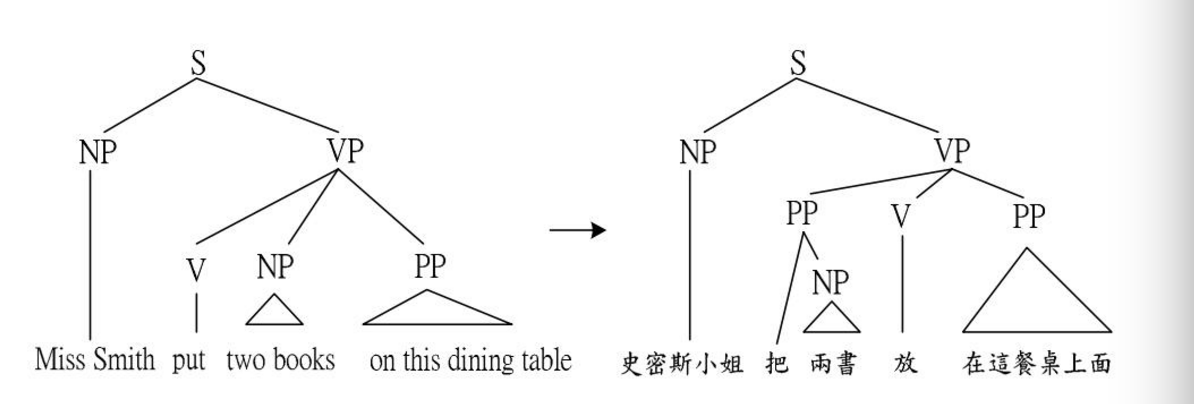
\includegraphics[width=9cm]{./rule-based-example}           % keine file extension angeben
		\caption{Example of rule-based translation process}  % Bild_unter_schrift
		\label{Rule_based_example}
	\end{center}
\end{figure}


\subsection{Stastical-based Translation}
The basic idea of statistical approach is to obtain translation rules and probability parameters automatically from bilingual corpus by employing statistical machine learning technologies. Graphic 1 shows string-based and tree-based translation model, which are used in statistical translation widely. Phrase-based model is a mature tranlation approach. The phrase means successive word sequences rather than the phrase defined in linguistics.

\begin{figure}
	\begin{center}
		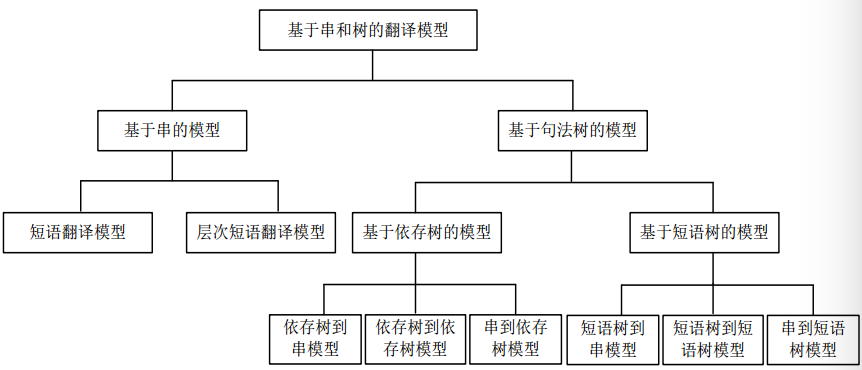
\includegraphics[width=9cm]{./statistical_translation_graph}           % keine file extension angeben
		\caption{string-based and tree-based translation models}  % Bild_unter_schrift
		\label{string-based and tree-based translation models}
	\end{center}
\end{figure}

\section{Neural Nerwork}

\section{Neural Machine Translation}

\section{Attention-based Neural Machine Translation}

\section{Evaluation}








\section{Introduction}
\label{sec:Abschnitt-1}

%% Der Befehl \section{} erstellt den ersten Abschnitt. Unter-
%% abschnitte werden mit \subsection{} generiert. Mit dem \label
%% Befehl erzeugt man eine symbolische Marke auf den Abschnitt.
%% Will man spaeter im Text auf den ersten Abschnitt referenzieren,
%% so gibt man das wie folgt an:


Dies ist eine Referenz auf Abschnitt~\ref{sec:Abschnitt-1}


%% LaTeX uebernimmt damit automatisch die Nummerierung der Referenzen.
%% Der Vorteil liegt darin, dass wenn man irgendwann mitten im Text einen
%% neuen Abschnitt einfuegt, muss man nicht manuell alle Referenzen
%% erneuern. Das Verwenden solcher symbolischer Referenzen sorgt dann
%% selber fuer die korrekte Referenzierung
%%
%%
%% Es kann sein, dass beim Compilieren des TeX-Files folgende Warnung
%% ausgegeben wird
%%
%% 	LaTeX Warning: There were undefined references.
%%
%%
%%	LaTeX Warning: Label(s) may have changed. Rerun to get ...
%%
%% Einfach der Anweisung folgen und neu compilieren.



Erzeugen wir erst etwas Text, um uns mit der Schreibweise in \LaTeX\ 
vertraut zu machen. \LaTeX\ bricht selbst\"andig Zeilen und Seiten um.
Selbst in einem Neogloismus wie dem ziemlich langen Wort aus Michael
Endes zuletzt geschriebenem Buch \glqq Der
satanarch\"aol\"ugenialkoh\"ollische Wunschpunsch\grqq\ findet \LaTeX\ eine
gute Trennstelle. Manchmal ist es aber sinnvoll, selber eine
Trennstelle vorzugeben. Dies gibt man mit $\backslash-$ im Wort im
\TeX-File selbst an, also \zB Trenn$\backslash-$stelle.
%
%
%
\\ \ \\   		% das erzeugt eine Leerzeile



L\"asst man eine Zeile im \TeX-File frei so wird automatisch die
n\"achste Zeile einger\"uckt. Wem das nicht gef\"allt, der kann im
\TeX-File den Befehl $\backslash$\texttt{parindent0pt} auskommentieren
und das damit unterdr\"ucken. 
Text mit \"a, \"o, \"U, Stra{"s}e, Caf\'e.\\[4ex]



%% Betrachten wir nun die Erzeugung mathematischer Formeln. In LaTeX
%% wir zwischen dem Text-Modus und dem mathematischen Modus
%% unterschieden. Um im laufenden Text Formeln zu verwenden, benutzt
%% man die $...$ Umgebung, z.B. wie folgt:


Dies ist ein laufender-Text mit Einsteins Formel $E = m \cdot c^2 $.
%
%
%% Natuerlich sind auch kompliziertere Formeln realisierbar.
%% Setzen wir z.B. die geometrische Reihe in eine eigene
%% Formelumgebung. Dies leitet man mit \[ ... \]  ein
\\ \ \\
Eine etwas kompliziertere Formel:
\[
     a \Frac{1 - q^{n+1}} {1-q}  =  \sum_{i=0}^{n} aq^{n} \qquad
     \text{mit\ } \quad a,q \in \mathcal{R},  q \neq 1
\]
%% Das Prinzip eines solchen Formelaufbaus ist relativ einfach.
%% Zunaechst schreiben wir unser ersten Symbol a hin. Dann folgt
%% ein Bruch. Dieser wird mit dem Befehl \Frac{}{} erzeugt. In
%% das erste Paar geschweifter Klammern schreibt man den Zaehler
%% rein, in das zweite Paar schreibt man den Nenner rein. Der
%% Zaehler enthaelt einen Exponenten. Exponenten werden immer
%% mit ^{} beschrieben. Alles was man dann in die Klammern
%% schreibt, steht dann im Exponenten. Analog gibt es natuerlich
%% auch Indizes. Diese notiert man mit _{}
%%
%%
%% Dieselbe Notation verwendet man auch fuer das Summenzeichen
%% (analog fuer das Produktzeichen \prod
%%
%%
%% Mit dem Befehl \mathcal erzeugt man ein kaligraphisches R im
%% mathematischen Modus. Der Befehl \neq erzeugt ein Ungleichheits-
%% symbol. Es gibt zahlreiche weitere Befehle zum Editieren von
%% Formeln in LaTeX. Fuer eine Uebersicht schaue man in der Literatur
%% nach, die auf der Webseite genannt ist.
%%
%%
%% Will man Formeln durchnumerieren, so kann man die equation-array
%% Umgebung benutzen.
%%
%%
\\ \ \\
Nun folgt die Bayessche Entscheidungsregel:\\

\begin{eqnarray}
\label{eq:bayes-decision-rule}
        r(X) = \underset{w_1 \dots w_N}{\mbox{argmax}}
        \bigg\{Pr(w_1^N | x_1^T)\bigg\}
        \quad \mbox{mit} \quad
        Pr(w_1^N | x_1^T) = \Frac{Pr(x_1^T | w_1^N) \cdot Pr(w_1^N)}
                            {Pr(x_1^T)}
        \quad .
\end{eqnarray}
%% Um Formeln richtig einzuruecken kann in der equation array Umgebung
%% das & Symbol verwendet werden. Gleichzeitig wollen wir die
%% Nummerierung der Formel unterdruecken. Dies geht mit einem *
%%
\\ \ \\
Beispiel f\"ur ein lineares Gleichungssystem:\\
\begin{eqnarray*}
	a_{11} x_1 + a_{12} x_2 + a_{13} x_3 &=& y_1\\
	a_{21} x_1 + a_{22} x_2		     &=& y_2\\
	a_{31} x_1			     &=& y_3 
\end{eqnarray*}



%% Statt \text kann man auch den etwas allgemeineren Befehl \mbox im
%% mathematischen Modus verweden, um reinen Text darzustellen.



%%%%%%%%%%%%%%%%%%%%%%%%%%%%%%%%%%%%%%%%%%%%%%%%%%%%%%%%%%%%%%%%%%%%%%%%%%%%%%%
%
%
%               Abschnitt 2
%
%
%%%%%%%%%%%%%%%%%%%%%%%%%%%%%%%%%%%%%%%%%%%%%%%%%%%%%%%%%%%%%%%%%%%%%%%%%%%%%%%
\section{Neural Network}
\subsection{Unterabschnitt}

\section{Neural Machine Translation}

\section{Attention-based Neural Machine Translation}
\subsubsection{Unter-Unterabschnitt: Beispiel f\"ur Tabellen}


%% Tabellen werden mit der tabular Umgebung erzeugt. Mit der table
%% Umgebung werden wir unserer Tabelle zusaetzlich eine Ueberschrift
%% geben und ihr mit \label einen symbolischen Namen zuordnen. Der
%% Aufbau einer Tabelle ist wie folgt: zunaechst wird in das zweite
%% Paar geschweifter Klammern eingetragen, wieviele Spalten man
%% haben will (hier |l|c|r|  , also 3). Das l weist LaTeX an, dass
%% die Eintraege der Spalte 1 linkbuendig, die der Spalte 2 zentriert
%% und die Eintraege der Spalte 3 rechtsbuendig dargestellt werden.
%% Das Symbol  |  steht fuer einen vertikalen Trennstrich. Laesst
%% man diesen weg, so enthaelt die Tabelle an der entsprechenden
%% Stelle auch keine Trennlinie mehr. Der Befehl \hline erzeugt eine
%% horizontale Trennlinie und wird nach einem Zeilenumbruch \\
%% angegeben.

In der Umgebung zum Plazieren von Tabellen (und auch Grafiken) kann
man optional die Werte t, b, h und H verwenden. Damit lassen sich
Tabellen am oberen Rand (top), unten (bottom) und an der aktuellen
Position (here) plazieren. Je nach Seitenlayout funktioniert die
Angabe h nicht immer. Mittels H l\"asst sich dann die aktuelle
Position erzwingen.

\begin{table}%[H,h,t,b,p]
\begin{center}
\caption{Beispiel Tabelle} % Tabellen_�ber_schrift
\label{tab:beispiel}
\vspace{2ex}
\begin{tabular}{|l|c|r|}
\hline
links		&	zentriert	&	rechts  \\ \hline\hline
links2		&	zentriert2	&	rechts2 \\ \hline
XXXXXXXXXXX	& XXXXXXXXXXXXXXXXXXXXX	& XXXXXXXXXXXX  \\ \hline

\end{tabular}
\end{center}
\end{table}


\subsection{Unterabschnitt: Beispiel f\"ur Grafiken}
Grafiken werden \"ublicherweise mit dem (frei verf\"ugbaren) Programm
tgif erstellt. Alternativ hierzu l\"asst sich auch das Programm xfig
verwenden. tgif ist zwar nicht ganz einfach zu bedienen, stellt dem
(erfahrenen) Anwender aber wesentlich mehr M\"oglichkeiten zur
Gestaltung von Grafiken zur Ver\"ugung. Die Konvertierung der *.obj
Dateien nach encapsulated PostScript erfolgt \"uber die Kommandozeile mit
\begin{center}
	tgif \quad -print \quad -eps \quad $<$Datei$>$.obj
\end{center} 

\begin{figure}
\begin{center}
  \includegraphics[width=9cm]{./architektur}           % keine file extension angeben
  \caption{Architektur eines Spracherkennungssystems}  % Bild_unter_schrift
  \label{fig:Erkenner-Architektur}
\end{center}
\end{figure}



\newpage
Nun erzeugen wir mittels \textsc{Bib}\TeX\ eine
Literaturliste. Dazu erzeugen wir uns ein File namens
$<$Dateiname$>$.bib, dass denselben Dateinamen wie unser \TeX-File
hat. Dieses wird dann mit
\begin{center}
	bibtex \quad  $<$Dateiname$>$
\end{center}
compiliert. Die im laufenden Text vorkommenden symbolischen
Literaturverweise zeigen dann auf den entsprechenden Eintrag
im Literaturverzeichnis. Dies geschieht mit dem Befehl
$\backslash$cite\{\}. Das sieht dann \zB wie folgt aus.
\\ \ \\
Zitat aus \cite{Name:1991}, Zitat aus \cite{Ende:1989}, Zitat aus
\cite{Name:1996}. Wichtig ist, das zuerst das \TeX-File compiliert
wird und dann das \textsc{Bib}\TeX-File. Da sich dann die Referenzen
meist \"andern, ist ein erneutes Compilieren des \TeX-Files notwendig.
\\ \ \\
Es gibt zahlreiche style-files, mit denen man das Layout eines
Literaturverzeichnisses \"andern und die Darstellung der
Literatur-Refererenzen modifizieren kann.
\\ \ \\
Letzter Hinweis: \LaTeX-Neulinge sollten auch die Kommentare im
\TeX-File lesen.

\section{Evaluation}

\addcontentsline{toc}{section}{Literaturverzeichnis}
\bibliographystyle{plain}
\bibliography{ausarbeitung_vorlage}

\end{document}
